\documentclass[letterpaper, 12pt]{article}
\usepackage{graphicx} % Required for inserting images
\usepackage{textcomp}
\usepackage{fullpage}
\usepackage{amsmath}
\usepackage{xcolor}
\usepackage{float}
\usepackage{geometry}
\usepackage{biblatex}
\geometry{margin=1in}
\usepackage{enumitem}
\usepackage{microtype}
\usepackage{gensymb}
\usepackage{parskip}
\usepackage{tikz}
\usepackage{caption}
\usepackage{cancel}
\usepackage{nicefrac}


\usepackage{hyperref}
\hypersetup{
    colorlinks=true,        % Enable colored links
    linkcolor=teal,         % Set color for internal links
    citecolor=teal,         % Set color for citations
    filecolor=teal,         % Set color for file links
    urlcolor=teal           % Set color for URLs
}

\usepackage[version=4]{mhchem}

\title{Practice questions and explanations}
\author{BIOS 1006}
\date{Week 1}

\begin{document}

\maketitle

\section*{Important things to remember}
*that have applications and are not just pure memorization

\begin{itemize}
\item As pH increases, compounds become deprotonated (lose an H$+$).
\item Always start with full protonation when finding the pI of a peptide.
\item Amino acid properties are determined by the properties of their side chains (i.e. know the properties of functional groups!).
\end{itemize}

\section*{Lecture 1: Fundamentals}

\subsection*{Functional groups}

\subsubsection*{Question 1: Naming}
Name the following functional groups.

\begin{figure}[H]
\centering
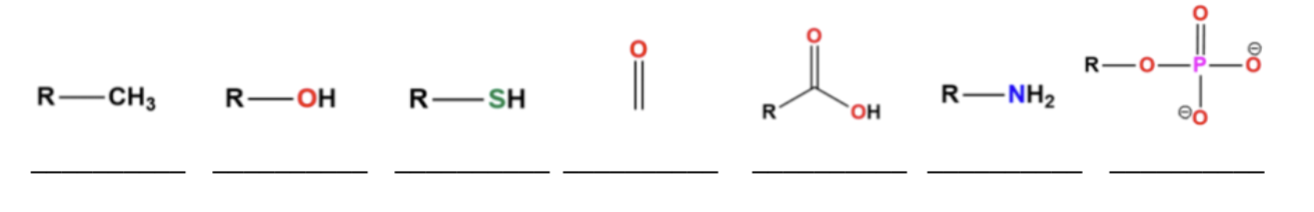
\includegraphics[width=0.9\textwidth]{functionalgroups}
\end{figure}

Answers:

\fbox{alkyl, hydroxyl, thiol (sulfhydryl), carbonyl, carboxyl, amino, phosphate}

Name the following linkages.

\begin{figure}[H]
\centering
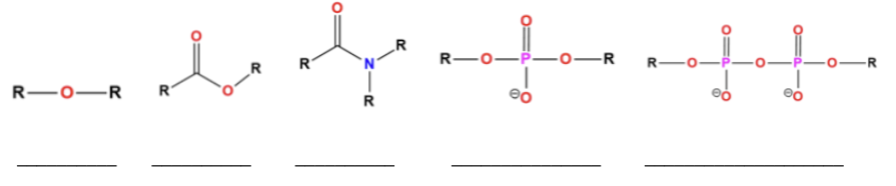
\includegraphics[width=0.9\textwidth]{linkages}
\end{figure}

Answers:

\fbox{ether, ester, amide, phosphodiester, phosphoanhydride}

\subsubsection*{Question 2: Roles of functional groups}

\begin{enumerate}
\item Amino acids and proteins have \fbox{amino} groups \& \fbox{carboxyl} groups.
\item Carbohydrates tend to have an abundance of \fbox{hydroxyl} groups and \fbox{ether} linkages.
\item Lipids vary greatly in structure, but fatty acids typically have \fbox{alkyl} groups.
\item Each nucleotide in a nucleic acid molecule has \fbox{phosphodiester} linkages.
\end{enumerate}

\subsection*{pH, pKa, pI}

\subsubsection*{Question 3: ICE tables and Henderson-Hasselbalch equation}

You make a 0.2 M aqueous solution of propionic acid \ce{CH3CH2COOH} by dissolving an appropriate amount of propionic acid in water. The pH of the resulting solution is 4.88. What is the pKa of propionic acid?

$$\ce{CH3COOH \rightleftharpoons CH3COO- + H+}$$

Set up the ICE table:

\begin{table}[H]
\centering
\begin{tabular}{c|c|c|c}
& \ce{[CH3COOH]} & \ce{[CH3COO-]} & \ce{[H+]} \\\hline
Initial & 0.2 & O & O \\
Change & -x & +x & +x \\
Equilibrium & 0.2-x & +x & +x \\
\end{tabular}
\end{table}

Given that the concentration of \ce{H+} is equal to x, we can undo the logarithm to find [\ce{H+}]:

\begin{gather*}
\text{pH} = -\log[\ce{H+}] \\
4.88 = -\log[\ce{H+}] \\
[\ce{H+}] = 1.32 \times 10^{-5} \: \text{M}
\end{gather*}

Now plug this into the Henderson-Hasselbalch equation:

\begin{gather*}
4.88 = pK_a + \log\left(\frac{1.32 \times 10^{-5}}{0.2-1.32 \times 10^{-5}}\right) \\
4.88 = pK_a + \log(6.6 \times 10^{-5}) \\
4.88 = pK_a - 4.18 \\
pK_a = 4.88 + 4.18 \\
pK_a = \boxed{9.06}
\end{gather*}

\subsubsection*{Question 4: Calculating pI of a peptide}

A tripeptide formed from tyrosine, valine, and glycine, in the order as stated. Use the following pKa values: $\alpha$-COOH = 2.2, $\alpha$-\ce{NH3+} = 9.4, tyrosine side chain OH = 10.5.

\begin{itemize}
\item[(a)] Draw the tripeptide and clearly label where the N-terminus and C-terminus are at pH 7.

$$ \text{(N-term)} \: \ce{NH3+ - Tyr - Val - Gly - COOH} \: \text{(C-term)} $$

\item[(b)] Calculate the charge of this tripeptide at pH 7.

Compare pKa and pH of each ionizable group:

N-term pKa 9.4 $>$ pH 7 $\rightarrow$ protonated, charge = +1

C-term pKa 2.2 $<$ pH 7 $\rightarrow$ deprotonated, charge = -1

Tyrosine side chain pKa 10.5 $>$ pH 7 $\rightarrow$ protonated, charge = 0 (protonated form, -OH, carries neutral charge)

\fbox{Overall charge: 0}

\item[(c)] Calculate the pI of this tripeptide at pH 7.

Order all the pKa values:

C-term 2.2 \\
N-term 9.4 \\
Tyr 10.5 \\

Always assume full protonation at the beginning (pH $<$ pKa). When the molecule is fully protonated, the overall charge is +1 (neutral C-terminus and tyrosine, positive N-terminus). As the pH increases, the C-term deprotonates first (pKa 2.2), then the N-term (pKa 9.4), and finally the side chain of tyrosine (pKa 10.5). The pI is the average of the two pKa values that surround the zero charge state.

+1 \\
C-term 2.2 \\
0 \\
N-term 9.4 \\
-1 \\
Tyr 10.5 \\
-2

The flanking pKas at charge 0 are 2.2 and 9.4.

$$ \frac{2.2 + 9.4}{2} = 5.8 $$

The pKa at pH 7 of the peptide is \fbox{5.8}.

\item[(d)] Will you be able to use UV light absorbance at 280 nm to detect your tripeptide? Why or why not?

\fbox{Yes, because the tripeptide contains a tyrosine side chain}, which has a phenolic ring that absorbs UV light at 280 nm. The other two amino acids (valine and glycine) do not absorb UV light at this wavelength.

\end{itemize}

\section*{Lecture 2: Amino acids and peptides}

\subsubsection*{Question 5: Amino acid chemical properties}

\paragraph{Which amino acid side chains are ionizable?} YECDHKR

\paragraph{Which amino acid has no chiral center?} G

\paragraph{Which amino acids have hydrophobic (nonpolar) side chains?} AVLIGMPFWY

\paragraph{Which amino acid side chain has an amino group?} K

\paragraph{Which amino acids have basic functional groups?} RHK

\section*{Lecture 3: Protein structure}

sadly i can't find anything worth putting here BUT KNOW DIHEDRAL ANGLES!!!

\section*{Lecture 4: Lab techniques}

\subsubsection*{Question 6: Protein purification}

You are attempting to purify the protein a-antitrypsin from a crude cell lysate in which
the main contaminants are the other four proteins, B-E, in the table below. The proteins
have the molecular weights (MW) and isoelectric points (pI) values shown in the table.
Each of the five proteins contains just a single polypeptide chain.

\begin{table}[H]
\begin{tabular}{|c|c|c|}
\hline
\textbf{Protein} & \textbf{Molecular weight} & \textbf{pI} \\\hline
A. $\alpha$-antitrypsin & 45,000 & 3.4 \\\hline
B. cytochrome c & 13,400 & 10.6 \\\hline
C. myoglobin & 17,000 & 7.0 \\\hline
D. serum albumen & 69,000 & 4.8 \\\hline
E. transferrin & 90,000 & 5.9 \\\hline
\end{tabular}
\end{table}

\begin{itemize}
\item [(a)] Which protein (A to E) will bind to cation-exchange resin at pH 7.4?

B, because pH $<$ pI, so the molecule is positively charged.

\item [(b)] Which protein (A to E) would elute first in size-exclusion chromatography?

E, because it has the highest molecular weight.
\end{itemize}

\end{document}